\documentclass[sigconf]{cidr-2027}

\title{Tail-Robust Query Planning from Triple Storage}

\author{Huahai Yang}
\affiliation{%
  \institution{Juji, Inc.}
  \city{San Jose, CA}
  \country{USA}}
\email{huahai.yang@gmail.com}

\renewcommand{\shortauthors}{Huahai Yang}

\begin{document}

\begin{abstract}
Triple stores complicate cost-based query optimization because predicates on a
single entity are correlated and relationship fanout depends on traversal
direction. Datalevin \cite{datalevin} addresses these challenges with a
layered strategy: index-maintained base-cardinality counts from nested
entity--attribute--value (EAV) and attribute--value--entity (AVE) indexes;
query-local reservoir sampling for conditional selectivity; and
regularization toward durable storage statistics.

On a 277.9-million-triple instance of the 113-query Join Order Benchmark
(JOB) \cite{leis2015optimizers}, a reference run supplied the same optimizer
with exact cardinalities (Exact). Full's median paired execution-time ratio
to Exact was $1.086\times$ (95\% CI [1.044, 1.160]). In the layer ablations,
each sampled condition used 30 paired seeds per query (3,390 trials). Shrinkage
lowered Raw's P99 from $12.26\times$ to $2.64\times$
(paired reduction $9.62\times$; 95\% CI [2.69, 11.29]), while the observed
count of Raw executions at or above $10\times$ fell from 48 to eight.
Hiding predicate counts caused 30 timeouts and removing query-local sampling
caused 80; Full had no timeouts in either experiment.
\end{abstract}

\begin{CCSXML}
<ccs2012>
 <concept>
  <concept_id>10002951.10003152.10003153.10010820</concept_id>
  <concept_desc>Information systems~Query optimization</concept_desc>
  <concept_significance>500</concept_significance>
 </concept>
 <concept>
  <concept_id>10002951.10003152.10003153</concept_id>
  <concept_desc>Information systems~Database query processing</concept_desc>
  <concept_significance>300</concept_significance>
 </concept>
 <concept>
  <concept_id>10002951.10003152.10003166</concept_id>
  <concept_desc>Information systems~Database management system engines</concept_desc>
  <concept_significance>300</concept_significance>
 </concept>
</ccs2012>
\end{CCSXML}

\ccsdesc[500]{Information systems~Query optimization}
\ccsdesc[300]{Information systems~Database query processing}
\ccsdesc[300]{Information systems~Database management system engines}

\keywords{Datalog, query optimization, cardinality estimation, sampling,
robust query processing, entity-attribute-value storage}

\maketitle

\section{Introduction}

Datalevin combines the declarative Datalog query language
\cite{maier2018datalog} with a flexible triple model. It stores facts as
entity--attribute--value triples $(E,A,V)$ rather than fixed-width rows, so
applications can add attributes without schema migrations and traverse
relationships in either direction.

EAV poses distinct optimization challenges. A \emph{reference attribute}
stores another entity's ID as its value and therefore represents a
relationship. A single logical entity spans many EAV triples, so queries over
several entity types initially resemble self-joins, with reference attributes
and ordinary value predicates interleaved. The relationship's fanout---the
number of output tuples per input---depends on whether traversal follows the
forward or reverse order.

The optimizer must estimate three quantities: attribute-predicate selectivity,
within-entity correlations, and directional relationship fanout. In a row
store, each histogram describes one typed column; in EAV, all domains share
the $V$ position and differ only by $A$, so a single $V$ histogram would mix
unrelated distributions. Per-attribute histograms avoid that mixing yet remain
marginal: they cannot capture predicate co-occurrence or fanout conditional on
the entities matched by earlier query steps. Precomputing statistics for
open-ended attribute combinations and traversal directions is expensive and
can lag the durable database. Triple-store systems accordingly replace
one-dimensional histograms with RDF-specific synopses or live-index sampling
\cite{neumann2010rdf3x,erlingVirtuoso}.

\begin{figure*}[t]
  \centering
  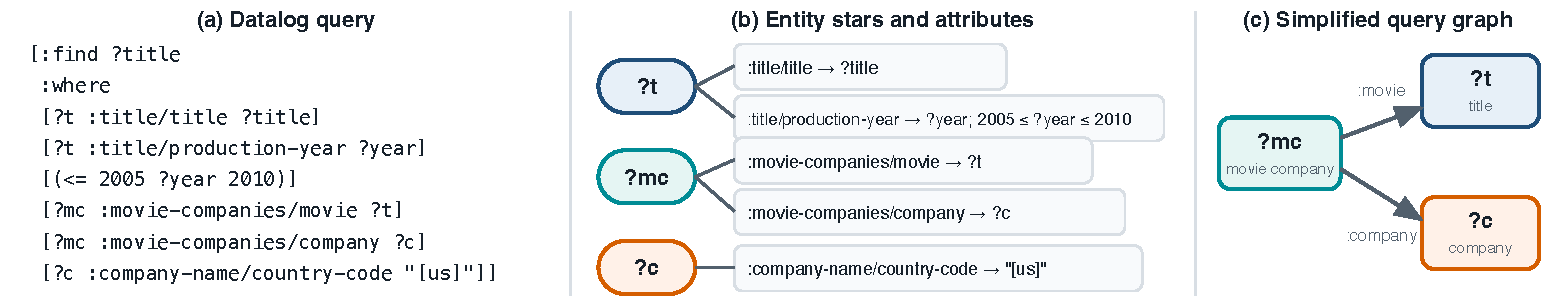
\includegraphics[width=\textwidth]{figures/query-graph.pdf}
  \caption{Illustrative query. (a) Datalog query. (b) Patterns grouped by
  entity variable into stars with attribute, value, and constraint spokes.
  (c) Collapsed query graph; stored references may be traversed in either
  direction.}
  \Description{Three panels show a Datalog query, its patterns grouped into
  three entity stars centered on variables t, mc, and c, and a simplified
  three-node graph. The title star has title and production-year attributes,
  the movie-company star has movie and company reference attributes, and the
  company star has a country-code attribute. Directed edges lead from the
  movie-company node to the title and company nodes.}
  \label{fig:query-graph}
\end{figure*}

Datalevin instead derives cardinalities from its storage structure and query execution
paths (Figure~\ref{fig:architecture}). Nested ordered indexes supply
index-maintained base counts at $O(\log n)$ cost. Query-specific samples are drawn
during planning from the entity ranges and traversal directions the query
induces, not from a global precomputed sample; the optimizer obtains them by
executing bounded versions of candidate scans and traversals.

An unlucky sample can cross a cost boundary where two join orders reverse.
Datalevin combines the query-local sample with a durable fanout prior:
shrinkage blends their means, while the production envelope takes their maximum.
The central claim is compositional: counts, sampling, and uncertainty
management address different dominant sources of execution-time tail, and
removing any layer reintroduces severe failures.

This system experience paper makes three contributions:

\begin{enumerate}
  \item A layered Datalog-planning architecture in which index-maintained counts
  resolve base cardinalities and query-local directional samples estimate
  correlation and fanout.
  \item Two lightweight, storage-aware policies---prior shrinkage and a
  conservative envelope---that reduce the risk of sample-induced bad plans
  without offline learning or conventional histograms.
  \item An ablation of counts, sampling, and regularization across all 113 JOB
  queries, with paired deterministic samples, plan-stability measurements,
  and execution-time tails, together with an exact-cardinality calibration of
  the fixed optimizer.
\end{enumerate}

Sections~\ref{sec:optimizer} and~\ref{sec:evidence} describe the optimizer and
its cardinality evidence; Section~\ref{sec:evaluation} evaluates the design.

\section{Optimizer Design}
\label{sec:optimizer}

Datalevin stores triples in two orders. Entity--attribute--value (EAV)
sorts by entity, then attribute, then value; this clusters each entity's
attributes together for efficient merge scans. Attribute--value--entity (AVE)
sorts by attribute, then value, then entity, forming a secondary index for
reverse-reference and value-equality lookups.

\noindent\textbf{Illustrative query.}
Figure~\ref{fig:query-graph}(a) shows a simplified JOB query in Datomic-style
Datalog \cite{datomicQueryStats} that returns US-produced movie titles from
2005 to 2010. Each where clause pattern matches an $(E,A,V)$ triple.
Patterns sharing an entity variable form an \emph{entity star}.
Figure~\ref{fig:query-graph}(b) shows these stars; collapsing them yields the
optimizer graph in Figure~\ref{fig:query-graph}(c), whose edges are reference
patterns.

On this entity-centered query graph, the optimizer applies cost-based dynamic
programming. It estimates cardinalities for each candidate expansion and
compares both indexed traversal directions, assembling a left-deep physical
plan that joins one new star at a time to the accumulated prefix.

\subsection{Entity stars and merge scans}

Patterns sharing an entity variable are not independent relations---they are
co-located in storage. In the example, the title and year patterns, together
with the range constraint, form the \texttt{?t} star. Datalevin's merge scan
walks candidate entity IDs in order and scans their requested attributes,
applying predicates on the fly. Like the RDF pivot index scan
\cite{brodt2011resource}, it produces one relation for the logical object
rather than materializing one relation per attribute.

Star collapse turns dozens of triple patterns into a smaller graph whose
nodes are stars and whose edges are references or shared values. The optimizer
chooses a starting star, then an order and direction for crossing the edges;
the example has three possible starts and two bidirectional edges.

\subsection{Plan enumeration}

The entity-star graph feeds plan enumeration. Datalevin applies
Selinger-style dynamic programming over connected subsets of each query-graph
component \cite{selinger1979access,moerkotte2008dynamic}.
It produces left-deep trees: each indexed expansion demands a base relation,
so bushy plans are not considered. Disconnected components are planned
independently, in parallel.

The enumerator preserves ordered keys and covers every connected ordered pair
of stars, hence every valid start and first traversal. Once the candidate
count for an $n$-star component exceeds $n(n-1)$, it retains only the cheapest
plan per connected, unordered star set.

\subsection{Physical alternatives}

Enumeration fixes the traversal order, but the optimizer must also choose
how each edge executes. The alternatives most relevant here are reference
traversals. A forward reference feeds target entity IDs directly into a merge
scan, whereas a reverse reference probes AVE to recover source entity IDs.
These two physical directions implement the same logical edge but can differ
sharply in cost and fanout; the estimator therefore treats them separately.

\subsection{Cost model}

Each candidate plan carries an estimated output cardinality and accumulated
cost. Base cost scales with the number of candidates entering the initial
index access and entity-star merge scan; pushed predicates and functions add
fixed per-tuple factors. Extending a prefix through a reference adds
$c_{\mathrm{probe}}N_{\mathrm{in}}+
c_{\mathrm{retrieve}}N_{\mathrm{out}}$, while a hash join is proportional to
the combined input sizes. These dimensionless operator weights rank plans.
The optimizer chooses the lowest
accumulated cost, using estimated output size to break ties.

Cardinality error cascades: $N_{\mathrm{out}}$ determines the current retrieval
cost and becomes $N_{\mathrm{in}}$ for later steps.
Underestimating a link can therefore make an expansion and its entire suffix
appear cheap, displacing a selective filter to a later position. The three
cardinality layers described in Section~\ref{sec:evidence} target precisely
these cost-model inputs.

\section{Managing Cardinality Uncertainty}
\label{sec:evidence}

\begin{figure*}[t]
  \centering
  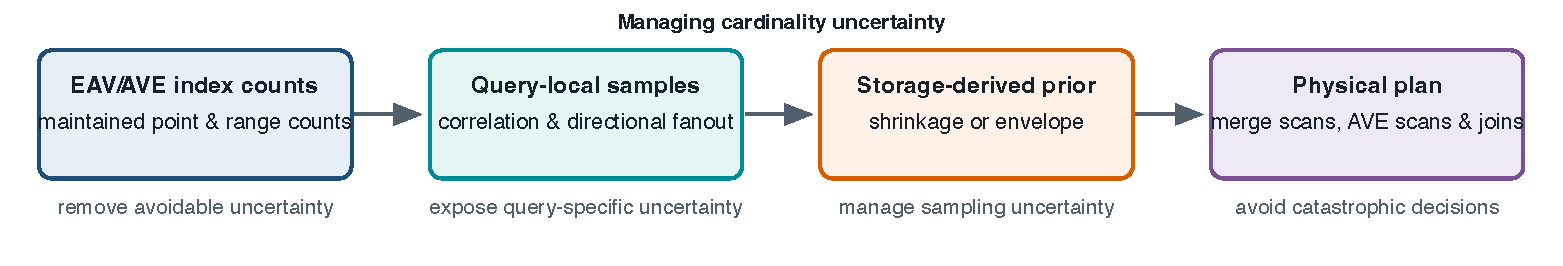
\includegraphics[width=\textwidth]{figures/architecture.pdf}
  \caption{The architecture for managing cardinality uncertainty. Counts
  resolve marginal cardinalities; samples estimate query-local correlation
  and directional fanout; the uncertainty policy regularizes those estimates
  before plan selection.}
  \Description{A left-to-right pipeline from EAV and AVE index counts,
  through a query-local directional sample and a storage-prior uncertainty
  policy, to a physical-plan decision.}
  \label{fig:architecture}
\end{figure*}

\subsection{Nested ordered indexes}

EAV and AVE also provide cardinalities. A literal triple representation would
repeat long shared prefixes, so Datalevin uses the
LMDB \texttt{DUPSORT} facility \cite{chu2011mdb},
which maps one key to an ordered value list. Conceptually, this is a nested
B$^+$ tree: the outer tree stores a shared index prefix, while an inner
ordered tree stores the remaining triple components. Separately, Datalevin's
underlying storage applies prefix compression within each page to remove
redundancy among neighboring encoded values. Internal nodes carry subtree
entry counts, supporting $O(\log n)$ count and rank operations.

For an AVE point predicate \texttt{[?e :a v]}, the number of entities is the
list count at key \texttt{(:a,v)}; rank metadata gives interval cardinality in
logarithmic time. EAV similarly counts a known entity and attribute. For an
attribute $a$, the durable prior
$\mu_0(a)=|\{(e,a,v)\}|/|\{v:\exists e\ (e,a,v)\}|$ is the mean AVE
postings-list length: expected source entities per distinct value. It is the
prior used in Section~\ref{sec:uncertainty} for AVE reverse-reference and
value-equality paths; forward references use EAV and are costed separately.
Unlike periodic histograms, these counts are updated with index entries in the
same LMDB transaction; copy-on-write MVCC publishes counts and entries
atomically to each reader snapshot, avoiding refresh lag. Datalevin also
verifies a reported zero against the index before using it to prove emptiness.

\subsection{Predicate pushdown and base cardinalities}

The compiler rewrites single-variable inequalities as index bounds, pushes
eligible functions into attribute scans, and substitutes constants before
planning. The count and scan therefore cover the same restricted range,
avoiding a mismatch between estimated and executed predicates.

For a fixed attribute $A$, a bound clause fixes $V$ to a constant; a free
clause leaves $V$ variable. Within each star, the optimizer uses
the pattern with the smallest index-counted base cardinality for the initial
scan and retains the alternatives. Small scans may execute during planning;
large ones use a bounded sample.

\subsection{Query-local directional sampling}

Counts establish marginal selectivity, but do not reveal whether several
attributes co-occur on the same entities or how many targets a relationship
reaches. For a range of $M$ candidates, Datalevin draws at most $m=1{,}000$
ranks uniformly without replacement and retrieves only those entries
\cite{vitter1985random}. Rank access costs $O(m\log M)$, or $O(\log M)$ in
database size for fixed $m$.

Sampled entity IDs pass through the same merge scan and
predicates that execution will use. The surviving fraction estimates the
selectivity of the complete star, including local correlations.

Relationship estimates are directional. If a reference links $A$ to $B$,
forward expansion, reverse lookup, and value equality can have different
fanouts. The estimator samples the candidate direction and access path. For
$n$ inputs, let $x_i$ be the joined outputs from input $i$, including zero for
no match. Directional join sampling produces the raw \emph{link ratio}
\[
  \widehat{r}^{\,\mathrm{raw}}_{A\rightarrow B}
  = \frac{\text{sampled join outputs}}{\text{sampled inputs}}
  = \frac{1}{n}\sum_{i=1}^{n}x_i
  = \bar{x}.
\]
This ratio predicts the multiplicative cardinality change along that physical
direction: a value below 1 is selective, 1 is cardinality-preserving, and a
value above 1 expands the input. The reverse ratio
$\widehat{r}_{B\rightarrow A}$ may be entirely different.

Sampling occurs at the base-plan stage; the optimizer caches star
selectivities and adjacent link ratios for use in deeper prefixes, where a
link maps $N$ estimated rows to $N\widehat{r}$. This assumes earlier joins do
not select a different-fanout subpopulation; deeper resampling showed little
development benefit.

Rare heavy hitters may be missed or overrepresented, and a noisy mean can put
an estimate on the damaging side of a plan-cost crossover.

\subsection{Storage-aware policies for sampling uncertainty}
\label{sec:uncertainty}

Given a sampled directional link ratio $\bar{x}$ and the attribute's durable
average fanout $\mu_0$, the unregularized baseline is
\[
  \widehat{\mu}_{\mathrm{raw}} =
  \max\!\left(\bar{x},\,\mu_{\min}\right).
\]
Here $\mu_{\min}=1.0$ is a conservative optimizer floor: it never credits a
sampled relationship traversal with reducing cardinality. This encodes the
asymmetric cost of estimation errors---overestimation is usually tolerable,
whereas underestimation can select a catastrophically bad join order. Raw
preserves query-local evidence without accounting for sampling uncertainty.
Against this baseline, we evaluate two policies that use the same reservoir
sample but manage its uncertainty differently.

\paragraph{Shrinkage.}
The first policy moves the raw mean toward the durable average fanout:
\begin{equation}
  \widetilde{\mu} =
  \frac{n\bar{x} + k_{\mathrm{eff}}\mu_0}
       {n+k_{\mathrm{eff}}},
  \qquad
  k_{\mathrm{eff}} = k(1+\alpha\,\mathrm{CV}^2).
  \label{eq:shrinkage}
\end{equation}
Here $k$ is the base strength of the storage prior, measured as an equivalent
number of observations. $\mathrm{CV}^2$ is the sample's squared coefficient of
variation, $\widehat{\mathrm{Var}}(x)/\bar{x}^2$ for $\bar{x}>0$ and zero
otherwise; $\alpha$ controls how strongly dispersion increases the prior
weight. Equation~\ref{eq:shrinkage} gives the sample weight
$n/(n+k_{\mathrm{eff}})$ and the prior weight
$k_{\mathrm{eff}}/(n+k_{\mathrm{eff}})$. A large, stable sample approaches
$\bar{x}$, whereas a small or dispersed sample moves toward $\mu_0$. The
final estimate is
$\widehat{\mu}_{\mathrm{shrink}}=\max(\widetilde{\mu},\mu_{\min})$.

\paragraph{Conservative envelope.}
The second policy takes a one-sided envelope over the query-local
observation and durable average:
\begin{equation}
  \widehat{\mu}_{\mathrm{env}} =
  \max\!\left(\bar{x},\,\mu_0,\,\mu_{\min}\right).
  \label{eq:envelope}
\end{equation}
The envelope cannot fall below either source of evidence.

For input cardinality $N$, the relationship estimate $N\widehat{\mu}$
propagates through later prefixes.
The envelope is no smaller than shrinkage because it takes a maximum rather
than an average. It is a decision rule, not an accuracy claim: underestimating
an expansion can move it ahead of selective work, while overestimating it
usually delays it. This may also postpone a beneficial traversal.

\section{Evaluation}
\label{sec:evaluation}

We ablate counts, sampling, and fanout policy (Table~\ref{tab:conditions}).
All conditions share the same plan space, physical alternatives, and operator
costs; only the named cardinality evidence or fanout rule changes. The primary
outcome is catastrophic slowdown; P95 and P99 summarize slowdown relative to
the corresponding Full-policy median. Full is the envelope condition. No
counts withholds predicate-specific point and range counts from costing but
retains $\mu_0$ metadata and physical sizes needed for correct execution or
sampling; equality falls back to $\mu_0$, other constraints to 10\% of the
attribute population. No sampling disables reservoir sampling of large base
ranges; small ranges may still execute exactly, and unsampled links use
$\mu_0$. Raw, Shrinkage, and Full receive identical sampled ranks within each
query-seed group, so their comparison isolates how the fanout rule interprets
the same evidence. A separate Exact reference, described in
Section~\ref{sec:exact}, calibrates Full without entering the layer ablation.

\begin{table}[H]
  \caption{Experimental conditions.}
  \label{tab:conditions}
  \centering
  \small
  \begin{tabular}{llll}
    \toprule
    Condition & Predicate counts & Sampling & Fanout policy \\
    \midrule
    Full        & Used   & Reservoir & Eq.~\ref{eq:envelope} \\
    Shrinkage   & Used   & Reservoir & Eq.~\ref{eq:shrinkage} \\
    Raw         & Used   & Reservoir & $\max(\bar{x},\mu_{\min})$ \\
    No sampling & Used   & None      & Durable prior $\mu_0$ \\
    No counts   & Hidden & Reservoir & Eq.~\ref{eq:envelope} \\
    \bottomrule
  \end{tabular}
\end{table}

\subsection{Setup and protocol}

JOB's 113 queries were designed to expose cardinality and join-order failures
on a large, highly correlated Internet Movie Database (IMDb) snapshot
\cite{leis2015optimizers}. We translated and verified the JOB workload in
Datalevin Datalog; \href{https://github.com/datalevin/datalevin/tree/cidr2027/benchmarks/JOB-bench/artifacts/cidr2027}{code and experiment artifacts are available online}.
The database contains 277,878,411 triples and occupies 17 GB.

Experiments ran on an Apple M3 Pro MacBook Pro with 36 GB memory and a 1 TB
SSD, using OpenJDK 21.0.11 and Datalevin 1.0.0.
On five development seeds, we compared candidate formulas and parameter
settings and selected the best-performing tested configuration ($m=1{,}000$,
$k=100$, $\alpha=0.4$). We then fixed it, along with the timeout and analysis
protocol, before the reported runs on disjoint seeds.
A post-confirmatory one-factor sensitivity run used ten seeds on 59 queries
whose Raw plans vary across seeds and on 20 stable controls, varying
$m\in\{250,1000,4000\}$, $k\in\{0,25,100,400\}$, and
$\alpha\in\{0,0.4,1.6\}$. The frozen point,
$(m,k,\alpha)=(1{,}000,100,0.4)$,
had no catastrophes; $m=4000$ or weaker regularization produced four to nine
(P99 $8.56$--$10.04\times$ versus the frozen $3.96\times$). This exploratory
run did not retune the reported conditions.

Full, No counts, Raw, and Shrinkage use 30 deterministic passes. Within each
pass, the harness shuffles all query--condition pairs with the pass seed, so
conditions are interleaved rather than run in batches. It also derives one
sample seed per query, shared across conditions. Because No sampling has one
deterministic plan, nominal seeds would be pseudoreplicates; it instead uses ten
randomized query-order schedules with paired Full controls. Sampled policies use
each query's 30-run Full median; No sampling uses its 10-run control median.

Each query--condition pair gets a fresh plan cache and a 30-second timeout,
charged at the limit. Queries run in a persistent, killable worker. After a
worker start or timeout-induced restart, the harness runs fixed query 6d and
two unmeasured replays of the next scheduled query before recording its time.
For every completed trial, it compares a result fingerprint---result
cardinality plus a hash of the returned value---across conditions and repeated
runs; all matched. Deterministic plan-only replays then use the same seeds to
record operator and traversal order without contributing timing observations.

Against paired Full controls, No sampling cut median preparation from 124.6 to
5.3 ms, but raised the median preparation-plus-execution time among completed
trials from 518 to 747 ms and timed out 80 times. We report these timing
numbers here rather than with the plan enumeration because the ablation
changes both the planning work and the plan it produces. A disjoint 100-seed
plan-only census covers all
113 queries, preserving identical ranks within each query-seed group.

For query $q$, trial $s$, and policy $p$, slowdown is
\begin{equation}
  S_{q,s,p} =
  \frac{T_{q,s,p}}
       {\operatorname{median}_{s'}T_{q,s',\mathrm{Full}}}.
  \label{eq:slowdown}
\end{equation}

\textbf{Catastrophe definition.} A trial is a catastrophe if it either reaches
the 30-second timeout or its runtime is at least $10\times$ the median
Full-policy runtime for the same query in the corresponding experiment
($S_{q,s,p}\geq 10$, Eq.~\ref{eq:slowdown}). Because the denominator is a Full median rather than
each Full observation, an individual Full run can also cross this threshold.
Reported 95\% intervals use 2,000 paired-bootstrap replicates that resample
queries and, within each resampled query, the seed-matched trials.

The 30-seed experiment has four queries (4c, 8c, 16b, and 17e) whose Full
median exceeds 3 seconds; the separate 10-schedule controls for No sampling
have seven (those four plus 10c, 13d, and 19d). For those query--experiment
pairs, the $10\times$ threshold lies beyond the timeout, so catastrophe is
equivalent to timeout. Table~\ref{tab:ablation} therefore separates completed
threshold crossings from timeouts. P95 and P99 remain query-relative: No
sampling's $461.098\times$ P99 comes from completed 31b runs of 3.86--3.88
seconds against an 8.394-ms Full median, not from a timeout.

\subsection{Exact-cardinality calibration}
\label{sec:exact}

Offline, a Datalevin-native factorized evaluator computed exact counts for
every connected entity-star subset and every indexed-link input, prior to
target-local filtering. Because all 113 JOB entity-star factor graphs are
acyclic, it streams star-local query factors and combines their multiplicities
by exact tree message passing over shared variables; link inputs combine
prefix multiplicities with exact AV-index point counts. This covers the
65,450 logical states and 103,961 distinct link-input count forms without
materializing candidate subplans. The checkpointed offline pass completed in
under one day.

Exact substitutes these counts without changing enumeration, pruning,
operators, or costs. We compare only execution times in 30 paired randomized
passes over all 113 queries (3,390 pairs), excluding preparation; all results
matched and no run timed out. Both bootstraps resample queries, then seeds:
the frozen ablation uses 2,000 replicates, while this later single contrast
uses 10,000 to reduce Monte Carlo error.

Full's median paired execution-time ratio to Exact was $1.086\times$ [1.044,
1.160]. Aggregating queries by their median paired ratio and applying the
original JOB study's buckets, 51.3\% of Full queries were within
$0.9$--$1.1\times$ of Exact, 20.4\% had at least $2\times$ slowdown, and none
reached $10\times$.

For scale, in the same JOB benchmark, PostgreSQL with primary- and
foreign-key indexes had 40\% of queries at least $2\times$ slower than
true-cardinality planning; that configuration also disabled non-index
nested-loop joins and enabled runtime hash-table resizing
\cite{leis2015optimizers}. Engines and protocols differ.

Six queries ran over 10\% faster under Full, so Exact is not a runtime lower
bound: the shared cost model can misrank wall-clock time and favor another
plan. Yet with search and costs fixed, the aggregate Full/Exact gap isolates
estimation headroom, and the dimensionless weights rank most JOB alternatives
usefully once counts are exact.

\subsection{Layer-by-layer ablation}

\begin{table}[t]
  \caption{Layer-by-layer ablation. $C_{\mathrm{run}}$ counts completed trials
  with $S\geq 10$, $C_{\mathrm{TO}}$ counts timeouts, and
  $C=C_{\mathrm{run}}+C_{\mathrm{TO}}$.}
  \label{tab:ablation}
  \centering
  \small
  \setlength{\tabcolsep}{4pt}
  \begin{tabular}{@{}lrrrrr@{}}
    \toprule
    Condition & $C_{\mathrm{run}}$ & $C_{\mathrm{TO}}$ & $C$ & P95 & P99 \\
    \midrule
    Full             & 4   & 0  & 4   & 1.425 & 2.883 \\
    Shrinkage        & 8   & 0  & 8   & 1.447 & 2.636 \\
    Raw              & 48  & 0  & 48  & 2.859 & 12.256 \\
    No sampling      & 176 & 80 & 256 & 93.455 & 461.098 \\
    No counts        & 127 & 30 & 157 & 6.780 & 30.059 \\
    \bottomrule
  \end{tabular}
  \begin{minipage}{\columnwidth}
    \footnotesize\emph{Note:} P95 and P99 are slowdown multiples relative to
    each condition's corresponding Full median. No sampling uses 10 randomized
    schedules per query (1,130 trials); all other conditions use 30 seeds per
    query (3,390 trials).
  \end{minipage}
\end{table}

\begin{figure}[t]
  \centering
  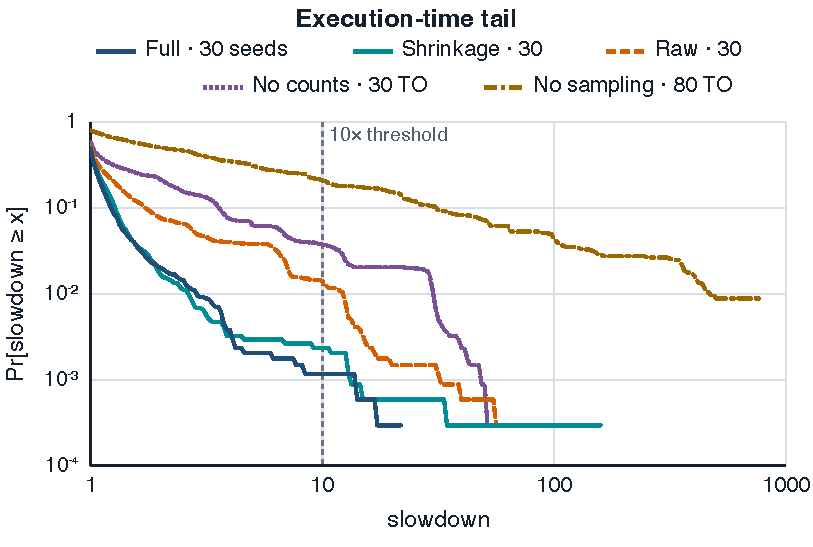
\includegraphics[width=\columnwidth]{figures/tail-ccdf.pdf}
  \caption{Complementary cumulative distribution function (CCDF) of slowdown
  relative to the corresponding Full median. Timeouts use the 30-second
  limit; TO denotes timeout.}
  \Description{Complementary cumulative slowdown curves for Full,
  Shrinkage, Raw, No counts, and No sampling. The plot marks the ten-times
  slowdown threshold and reports 30 No-counts and 80 No-sampling timeouts.}
  \label{fig:tail}
\end{figure}

\begin{table*}[t]
  \caption{Per-query catastrophe concentration. $Q_C$: affected queries;
  $C_{-1}=C-\max_q C_q$: count after dropping the largest contributor.
  Superscript \textsc{to}: every trial timed out; zero-count queries omitted.}
  \label{tab:query-concentration}
  \centering
  \scriptsize
  \setlength{\tabcolsep}{4pt}
  \renewcommand{\arraystretch}{1.03}
  \begin{tabular}{@{}lrrrrp{0.58\textwidth}@{}}
    \toprule
    Condition & $Q_C$ & $C$ & $\max_q C_q$ & $C_{-1}$ & Nonzero $C_q$ by query \\
    \midrule
    Full & 4 & 4 & 1 & 3 &
      23b, 27a, 29b, 33b (1 each) \\
    Shrinkage & 6 & 8 & 2 & 6 &
      22d, 31b (2 each); 1a, 1d, 14b, 21b (1 each) \\
    Raw & 8 & 48 & 30 & 18 &
      22d (30); 11d (8); 31b (4); 33c (2); 21a, 24b, 30b, 33a (1 each) \\
    No sampling & 31 & 256 & 10 & 246 &
      7b, 8c$^\mathrm{TO}$, 8d$^\mathrm{TO}$, 10c$^\mathrm{TO}$, 12a,
      15a, 15c$^\mathrm{TO}$, 15d, 18c, 19c, 22c, 22d,
      23a$^\mathrm{TO}$, 23c$^\mathrm{TO}$, 24b, 29a, 29b,
      30b$^\mathrm{TO}$, 30c$^\mathrm{TO}$, 31a, 31b, 31c, 33b (10 each);
      19a (8); 25c (6); 12c (4); 30a (3); 2b (2); 1c, 6a, 25b (1 each) \\
    No counts & 10 & 157 & 30 & 127 &
      6b, 17c, 25b (30 each); 8c$^\mathrm{TO}$ (30); 19a (15); 19c (13);
      24a (6); 10b, 21c, 33b (1 each) \\
    \bottomrule
  \end{tabular}
\end{table*}

Figure~\ref{fig:tail} shows No sampling with the broadest tail, followed by No
counts; Raw separates from Shrinkage and Full around $10\times$. Because No
sampling has fewer trials, its raw total understates the contrast:
256 of 1,130 trials (22.7\%) were catastrophes, versus 157 of 3,390
(4.63\%) for No counts.
The two failure sets overlap on five queries (8c, 19a, 19c, 25b, and 33b); No
sampling nevertheless affected 31 queries versus ten and produced the broader
tail.

Full's four threshold crossings occurred on 23b, 27a, 29b, and 33b. The
recorded structural plan recurred in 26 of 30 trials for 23b and all 30 trials
for each other query. After excluding the crossing, each same-plan median was
within 3.8\% of its original Full median; none of the four measurements followed
a worker restart. The stable plans make sample-induced plan failure unlikely,
but do not identify the physical cause: the harness did not record GC, thermal,
SSD, or scheduler counters. We retain all four without attributing them.

\textbf{Counts prevent severe base-cardinality errors.} No counts caused 157
catastrophes across ten queries; query 8c accounted for all 30 timeouts.
Of the 127 completed catastrophes, 125 changed operator or traversal order.
The 8c timeout concentration is consistent with a misranked starting star,
but Table~\ref{tab:query-concentration} shows that the result does not depend on
8c: dropping it leaves 127 catastrophes across nine queries, including 30
completed catastrophes each on 6b, 17c, and 25b.

\textbf{Query-local sampling prevents a correlation-and-fanout tail.} No
sampling produced 256 catastrophes across 31 queries; eight timed out in every
schedule (80 timeouts). The timeout tail is conservative because each timeout
contributes only the 30-second limit. Excluding those eight all-timeout queries,
176 completed catastrophes remain across 23 queries; dropping any single query
leaves at least 246 catastrophes. The fixed plan differed from Full in all ten
runs for 99 of 105 queries,
indicating systematic rather than timing noise.
Counts still provide marginal sizes, so the ablation jointly removes within-star
correlation and directional fanout. The durable average can then describe the
wrong subpopulation and make expansion appear safe too early.

\textbf{Regularization suppresses the sampling tail.}
Raw produced 48 catastrophes, 47 with a plan different from Full. Shrinkage
produced eight, five with a different plan, cutting P99 from $12.256\times$ to
$2.636\times$---a paired reduction of 9.620 [2.693, 11.288]. The
catastrophe-rate reduction was 1.180
percentage points, but its query-clustered confidence interval [0.000, 3.187]
includes zero. Storage evidence therefore sharply reduces the continuous
tail, though the clustered catastrophe-rate interval is inconclusive.

Because Raw and Shrinkage see identical sampled ranks, their difference comes
from interpretation rather than observations. Noisy means cross discrete cost
boundaries; optimistic fanout errors can move large expansions ahead of
filters, whereas moderate overestimates more often merely delay work.

\textbf{The envelope and shrinkage make different tradeoffs.} The envelope
produced four observed catastrophes versus eight for Shrinkage, but Full minus
Shrinkage in catastrophe rate was $-0.118$ percentage points [$-0.442$,
0.147]. Shrinkage had lower observed P99, but Full minus Shrinkage was 0.247
[$-0.690$, 1.574]. The envelope guards against estimates that fall below both
observation and durable average. Its simpler computation and lower observed
catastrophe count motivate the production choice.

In the census, departures from each query--condition modal plan occurred in
15.37\% of Raw trials, 11.40\% of Shrinkage trials, and 5.79\% of Full trials.
Thus storage-aware policies reduced seed sensitivity, with the envelope most
stable; the metric does not measure agreement with Full.

\section{Related Work}

Datalevin applies dynamic programming over connected subgraphs after
entity-star collapse \cite{selinger1979access,moerkotte2008dynamic}.

Datomic has related Datalog syntax but no cost-based join-order planner: except
for a few documented always-beneficial rewrites, it evaluates clauses in source
order \cite{datomicQueryStats}.

A row-store histogram is not the corresponding triple-store baseline. RDF-3X
found one-dimensional subject/predicate/object histograms inaccurate on its two
more complex datasets. Its effective alternative uses six order-specific
histograms with nine join-partner counts per bucket plus frequent-path
statistics \cite{neumann2010rdf3x}. Virtuoso likewise reports that generic SQL
statistics lose usefulness when RDF occupies one large table and instead
samples the live index during optimization \cite{erlingVirtuoso}. Both tie
evidence to triple indexes or graph structure.

Characteristic sets summarize predicates that co-occur on an RDF subject,
capturing correlations missed by one-dimensional marginals, but require
precomputation \cite{neumann2011characteristic}. Datalevin instead obtains
current, query-local evidence from its execution indexes.

Classical join estimators combine samples with frequent-value statistics to
handle skew \cite{haas1995sampling}. Index-based join sampling has also been
evaluated on JOB \cite{leis2017cardinality}, and learned estimators target
correlated joins \cite{kipf2019learned}. Our focus differs: repeated query-local
samples create a plan-tail problem, and our ablations isolate how index counts,
sampling, and storage-derived regularization control it.

Robust optimization seeks predictable performance under cardinality
uncertainty \cite{babcock2005robust}. Datalevin does not enumerate uncertainty
scenarios; it regularizes live evidence before ordinary plan search.

\section{Conclusion}

EAV flexibility need not preclude predictable cost-based planning. Index
counts prevent base-cardinality errors, query-local samples reveal conditional
selectivity and directional fanout, and regularization keeps noise from
crossing plan boundaries. Hiding counts caused 30 timeouts, disabling sampling
caused 80, and shrinkage lowered Raw's P99 from
$12.26\times$ to $2.64\times$ on identical ranks. With exact cardinalities,
the optimizer's median paired Full/Exact execution-time ratio was
$1.086\times$ [1.044, 1.160], exposing estimator headroom.

The production envelope was simplest and had the lowest observed catastrophe
count, though neither its catastrophe-rate nor P99 difference from shrinkage
was significant. One model, machine, and analytical workload limit
generalization; finite deterministic seeds characterize observed tail risk,
not a universal failure probability. Future work should target sampling near
plan-order thresholds and uncertain deeper joins.

\bibliographystyle{ACM-Reference-Format}
\bibliography{references}

\end{document}
